Esitellään palveluperustaisten web-sovellusten tunnistautumisen ongelmakenttää ja esitellään niihin suunniteltuja protokollia, aikajärjestyksessä kerberos -> saml -> oauth ja päädytään oauthiin, tarkemmin versioon 2.

Kappaleessa vedetään yhteen kappaleissa 2 ja 3 esiteltyjä perusjuttuja ja avataan nykyaikaisiin hajautettuihin web-sovelluksiin liittyviä tunnistautumisongelmia. Ratkaisuksi tarjotaan erilaisia protokollia ja tehdään niistä vertailua.

Pituus n. 10 sivua. Tämä on alkupään kappaleista oleellisin, koska tässä oikeasti pureudutaan ongelmaan, joka yrityksellä on.

Lähteitä:\\
A billion keys, but few locks: the crisis of web single sign-on \cite{billion_keys}\\
A large-scale study of web password habits \cite{password_habits}
Inside the identity management game \cite{inside_the_identity_management_game}\\
Decentralization: The Future of Online Social Networking \cite{decentralisations}\\
Lampson \& kumppanit: Authentication in distributed systems: theory and practice \cite{lampson}.

Kerberos:\\
Enhancing Distributed Web Security Based on Kerberos Authentication Service \cite{enchancing_distributed_web_security}\\
Secure Secret-Key Management of Kerberos Service \cite{secure_secret_key}\\
RFC4120 \cite{rfc4120}\\
RFC3244 \cite{rfc3244}

SAML:\\
Research of Dynamic Authentication Mechanism Crossing Domains for Web Services Based on SAML \cite{dynamic_saml}\\
Next steps for security assertion markup language (saml) \cite{next_saml}

OAuth:\\
2.0 draft: http://tools.ietf.org/html/draft-ietf-oauth-v2-22 \cite{oauth2_0}

-----------------------------------------------------------------------------------------------------------

Miten käyttäjädataa onko käsitelty ja käsitellään. Kehitys paikallisesti käytetyistä tiedostopohjaisista systeemeistä kohti tietokantoja ja asiaan räätälöihin palveluihin (LDAP). LDAP oleelisin, mutta tutkimuksen kannalta abstraktointi on tärkeä juttu.

Johdanto puoli sivua, alaluvut 0.5-1 sivu.
\subsection{Ongelmakenttä}
Palvelusuuntautuneissa web-ohjelmistoissa käyttäjien tunnistautuminen on toteutettu monin tavoin. Tyypillisesti kysytään käyttäjältä tunnus ja salasana, joita verrataan ohjelmiston paikalliseen käyttäjätietokantaan. Paikallinen tietokanta on kopioitu palvelun varsinaisesta käyttäjätietokannasta ja paikallisiin tietokantoihin on käyttäjille luotu erillinen käyttäjätunnus.

Tästä seuraa monenlaisia synkronointiongelmia. Esimerkiksi työntekijän irtisanoutuessa joudutaan tunnus poistamaan kaikista tietokannoista erikseen. Myös osoitteen yms. tietojen muutokset täytyy päivittää kaikkiin tietokantoihin. Lisäksi käyttäjälle syntyy saman järjestelmän sisällä monia tunnuksia, joihin saattaa liittyä erilliset salasanat. Käyttäjän kannalta on myöskin ikävää kirjautua jokaiseen osapalveluun erikseen.

\subsection{Ympäristö}
Yrityksen tai yhteisön web-sovellukset ovat avoimia pienemmälle osajoukolle käyttäjiä, esimerkiksi yrityksen intranet-järjestelmään on pääsy vain yrityksen työntekijöillä, jotka on kirjattu tietokantaan. Erilaisin palomuuri-asetuksin pääsy intranet-järjestelmään voidaan rajata vain yrityksen sisäverkkoon, mutta sekään ei poista tunnistautumisen tarvetta. Aivan kuin avoimissa sovelluksissa, myös intranet-järjestelmässä halutaan tietää kuka yrityksen työntekijöistä sitä kulloinkin käyttää, jotta työntekijälle osataan näyttää vain häntä koskevaa dataa.

Joissakin tapauksissa intranet-järjestelmä pitää sisällään myös käyttäjähallinnan, jolloin yrityksessä ei ole erillistä tietokantaa käyttäjille, vaan jokaiselle työntekijälle luodaan erillinen tunnus intranetiin. Toisissa tapauksissa taas halutaan hyödyntää erillistä käyttäjähallintaa, jolloin käyttäjän tiedot ovat  esimerkiksi erillisellä LDAP-palvelimella, jota vasten intranet-järjestelmä tunnistaa käyttäjät.

Palvelusuuntautuneissa arkkitehtuureissa samaa käyttäjätietokantaa käyttäviä sovelluksia, tai palveluita, voi olla useita. Tällöin ns. pääkäyttäjäkannasta voidaan luoda oma paikallinen kopio jokaista palvelua varten. Tästä seuraa monenlaisia synkronointiongelmia [TODO: lähde]. Esimerkiksi työntekijän irtisanoutuessa joudutaan tunnus poistamaan kaikista tietokannoista erikseen. Myös osoitteen yms. tietojen muutokset täytyy päivittää kaikkiin tietokantoihin. Lisäksi käyttäjälle syntyy saman järjestelmän sisällä monia tunnuksia, joihin saattaa liittyä erilliset salasanat. Käyttäjän kannalta on myöskin ikävää kirjautua jokaiseen osapalveluun erikseen.

Koko käyttäjäkantaa ei ole kuitenkaan tarve kopioida jokaiselle sovellukselle, vaan yksittäiset sovellukset voivat tunnistautua erillistä tunnistautumispalvelua vasten [TODO: lähde]. Tällöin käyttääkseen yrityksen intranet-palvelua, täytyy käydä tunnistautumassa tunnistautumispalvelussa. Nykypäivänä monet web-sovellukset toimivat juuri ulkoisen tunnistaumispalvelun kautta. Viihdesivustoille voi luoda tunnuksen kirjautumalla Facebookin tai LinkedInin kaltaisten sivustojen kautta [TODO: lähde?]. Myös esimerkiksi Kelan sivuston käyttöä varten tunnistaudutaan pankkitunnuksilla Tupas-järjestelmän avulla [TODO: lähde].

Palvelusuuntauneen arkkitehtuurin kannalta tunnistautumisen keskittäminen yhdelle palvelulle on kiinnostava idea. Tällöin yksittäinen palvelu käyttää tunnistautumiseen erillistä palvelua, joka integroituu yrityksen tai yhteisön käyttäjäkantaan. Keskitettyä tunnistautumista käsitellään seuraavassa luvussa.
\subsection{Käyttötapauksia}
kuva soa-palvelusta (abstraktoinnin tarve)
\subsection{Keskitetyn tunnistaumisen periaatteet}
Keskitetyn tunnistautumisen lähtökohta on käyttäjän tunnistetietojen poistaminen web-palvelun hallinnasta. Käyttäjä ei syötä tunnistetietojaan missään vaiheessa web-palveluun, vaan tunnistautuminen tehdään keskitetyssä paikassa. Nykyisin mm. Facebook ja Google tarjoavat julkiset API-rajapinnat, joiden avulla web-palvelut voivat käyttää niitä tunnistautumiseen.

Kuvassa \ref{facebook_login} on kuvattu kirjautuminen Porkkanamafia-ryhmän WWW-sivulle käyttäen Facebookia. Käyttäjä klikkaa WWW-sivulla olevaa "Login with Facebook" -nappia, jonka jälkeen käyttäjän selaimeen avautuu Facebookin varmennusikkuna, jossa käyttäjää pyydetään varmentamaan kirjautuminen. Selaimen osoitekenttä osoittaa käyttäjälle, että kirjautuminen tapahtuu nimenomaan Facebook-sivulla (joka on varmennettu SSL-sertifikaatilla), joten käyttäjän Facebook-tunnistetiedot eivät päädy Porkkanamafian haltuun, vaan kirjautuminen hoidetaan suoraan Facebookiin.

Kirjautumisen jälkeen käyttäjälle luodaan rivi käyttäjätietokantaan, jossa on viittaus hänen Facebook-tunnukseen. Tämän jälkeen, kun käyttäjä palaa sivulle, ja kirjautuu jälleen Facebook-tunnuksilla, voidaan Facebookilta tullut käyttäjä yhdistää kannasta löytyvään vanhaan käyttäjään. Näin palvelu on ulkoistanut tunnistautumisen ulkopuoliselle taholle, eikä käyttäjän tarvitse muistaa uusia tunnistetietoja, vaan hän voi käyttää Facebook-kirjautumista jatkossa.

\begin{figure}[ht]
\centering
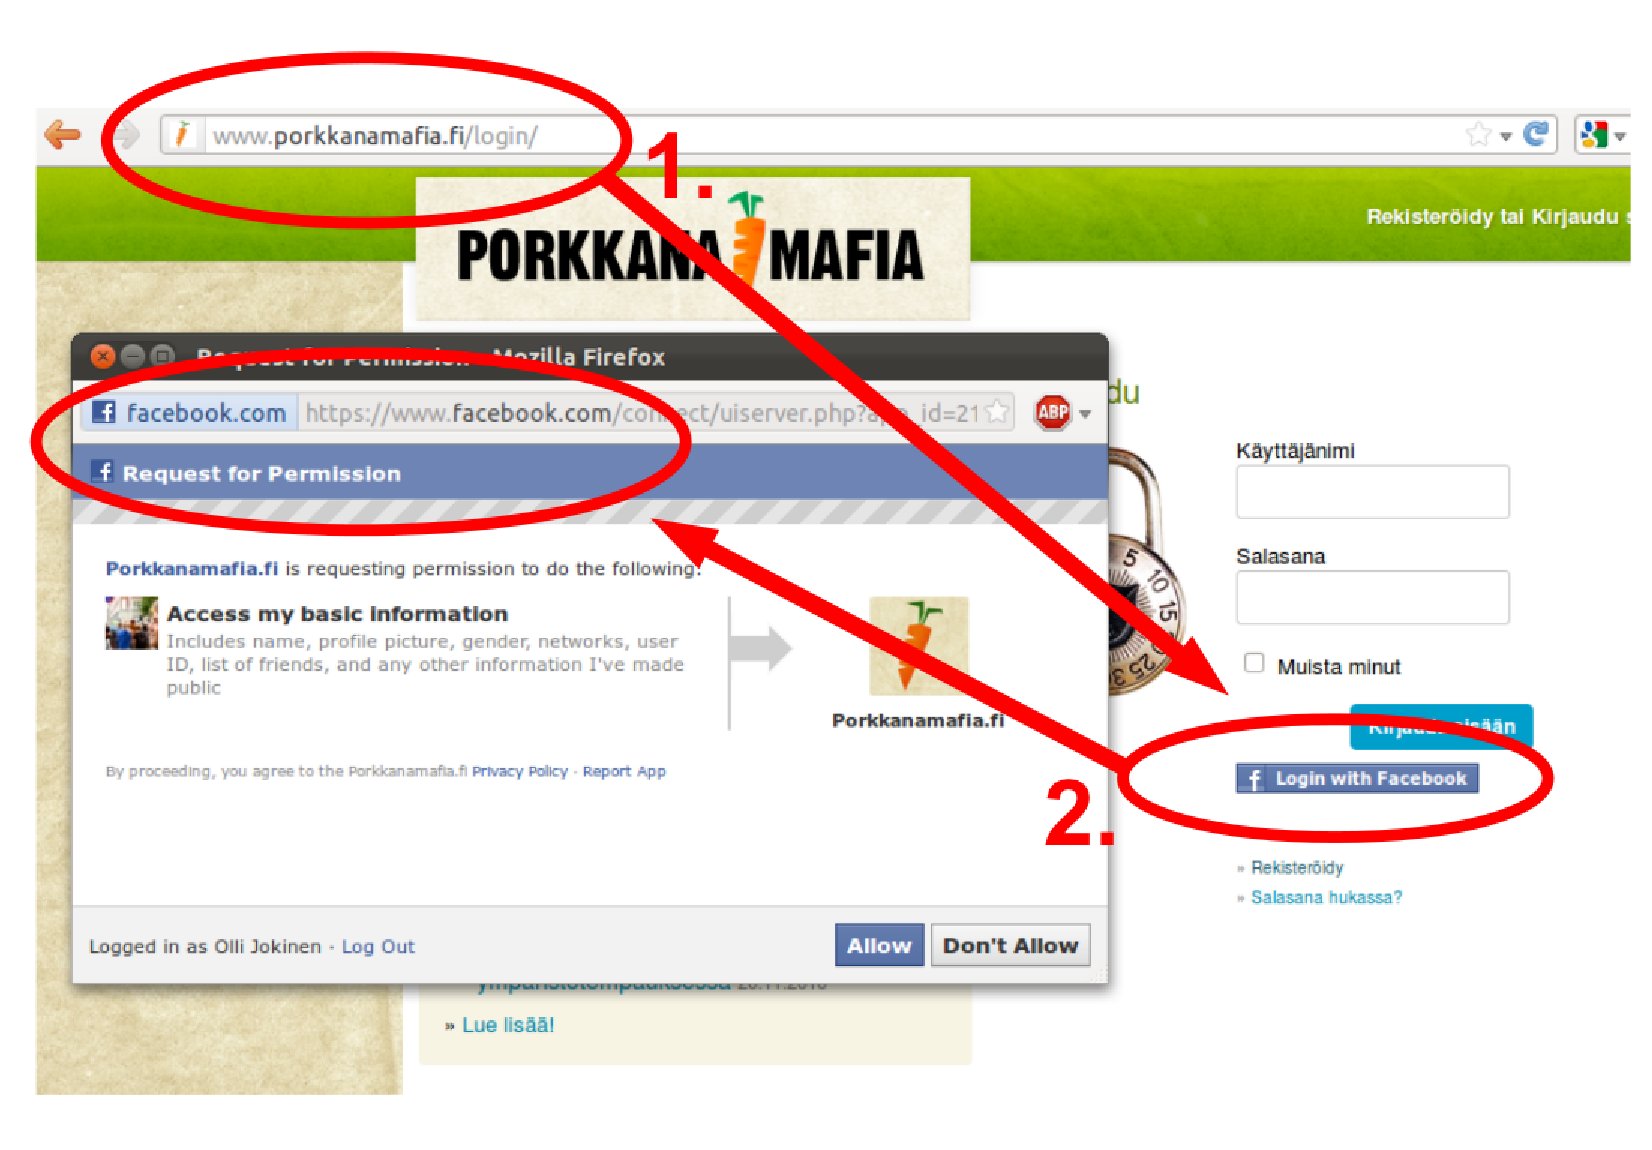
\includegraphics[width=\textwidth]{teknologiat/facebook.eps}
\caption{Käyttäjän kirjautuminen Facebook-tunnuksilla Porkkanamafian web-palveluun}%
\label{facebook_login}
\end{figure}

Samaa periaatetta voidaan käyttää myös organisaatioiden sisäisessä tunnistautumispalvelussa. Organisaation sisäiseen palvelusuuntautuneeseen arkkitehtuuriin toteutetaan erillinen web-palvelu, joka on yhteydessä olemassa olevaan käyttäjätietokantaan (esim. LDAP), ja tarjoaa Facebookia vastaavan tunnistautumisen.

Keskitetty tunnistautumispalvelun periaate on kuvattu kuvassa \ref{composition}, jossa on neljä palveluun kuuluvaa komponenttia. Ensimmäiseksi käyttäjä menee WWW-selaimen avulla web-palveluun, joka pyytää tunnistautumista erillisessä tunnistautumispalvelussa. Käyttäjän selain ohjataan tunnistautumispalvelun sivulle, joka on yhteydessä organisaation käyttäjähallintaan. Jos käyttäjähallinnasta löytyy käyttäjän syöttämät tunnistetiedot, palautetaan käyttäjälle valtuutusavain, jonka käyttäjä lähettää takaisin web-palvelulle. Tämän jälkeen web-palvelu varmistaa tunnistautumispalvelulta valtuutusavaimen oikeellisuuden ja tunnistautumispalvelu palauttaa käyttäjän tiedot web-palvelulle.

\begin{figure}[ht]
\centering
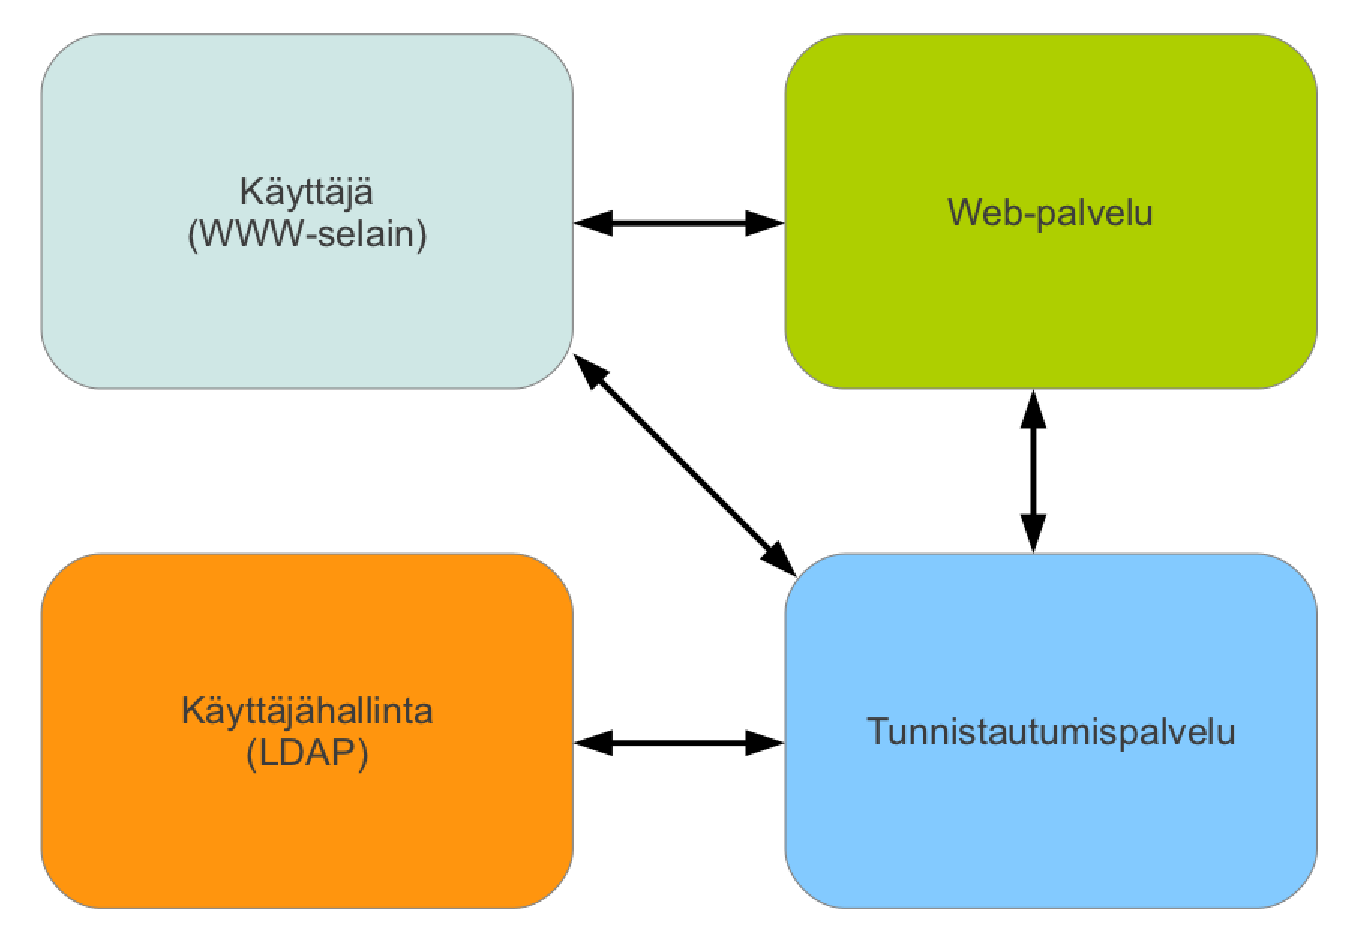
\includegraphics[width=\textwidth]{teknologiat/composition.eps}
\caption{Keskitetyn tunnistautumisen periaatteet}%
\label{composition}
\end{figure}

\subsection{Keskitetyn tunnistautumisen rajapintaprotokollat}
Miten käyttäjädataa onko käsitelty ja käsitellään. Kehitys paikallisesti käytetyistä tiedostopohjaisista systeemeistä kohti tietokantoja ja asiaan räätälöihin palveluihin (LDAP). LDAP oleelisin, mutta tutkimuksen kannalta abstraktointi on tärkeä juttu.

Johdanto puoli sivua, alaluvut 0.5-1 sivu.
\subsubsection{Kerberos}
Lähteet:
Enhancing Distributed Web Security Based on Kerberos Authentication Service (\cite{enchancing_distributed_web_security})
Secure Secret-Key Management of Kerberos Service (\cite{secure_secret_key})

Kerberos-protokolla on alunperin MIT:ssa kehitetty tunnistautumisprotokolla, jonka nykyisin käytössä oleva versio 5 julkaistiin alunperin syyskuussa 1993 ja päivitettynä heinäkuussa 2005 [RFC4120]. Se on yleisesti käytössä erilaisissa UNIX-pohjaisissa käyttöjärjestelmissä ja myös Microsoft on käyttänyt sitä oletus-tunnistautumismekanismina Windows 2000:sta lähtien [RFC3244].

Protokollan osapuolia ovat käyttäjä, luotettava kolmas osapuoli ja palvelu, joka vaatii tunnistautumisen. Luotettava kolmas osapuoli on tyypillisesti avaintenjakopalvelin (KDC, Key Distribution Center), joka tunnistaa käyttäjän ja myöntää lipun tunnistautuneelle käyttäjälle. Myönnettyyn lippuun on merkattu palvelu, johon sitä voidaan käyttää ja aikaleima, jonka ajan se on voimassa. Käyttäjä antaa lipun tunnistautumista vaativalle palvelimelle, joka tarkistaa omalla avaimellaan käyttäjän tunnisteen ja aikaleiman, joiden perusteella se myöntää pääsyn palveluun.

Keskitetty tunnistautuminen hajautettuihin järjestelmiin voidaan toteuttaa Kerberos-protokollalla \cite{enchancing_distributed_web_security}. Kerberos on luonteeltaan sopiva hajautettuihin järjestelmiin, koska avaintenjakopalvelin voi jakaa lippuja kaikkiin järjestelmiin, joiden kanssa se on vaihtanut salausavaimet. Tunnistautumispalvelin on tilaton, jolloin sen suorituskykyä voidaan parantaa tarvittaessa skaalaamalla, joten tunnistautumispalvelin voi palvella suurta määrää käyttäjiä \cite{enchancing_distributed_web_security}.

Tunnistautumisessa käytetyt yksityiset avaimet tallennetaan tietokantaan, jolloin on riskinä, että kolmas osapuoli saattaa päästä käsiksi näihin avaimiin ja pystyä allekirjoittamaan lippuja. Jakamalla salaiset avaimet osiin ja hajauttaa se avaintenjakopalvelimeen, tunnistautumista vaativalle palvelimelle ja näiden välillä käytetylle reitittimelle \cite{secure_secret_key}, voidaan parantaa protokollan luotettavuutta. Tämä tekee siitä mahdollisen vaihtoehdon käytetyksi menetelmäksi keskitettyyn tunnistautumiseen hajautetuissa järjestelmistä.

\subsubsection{SAML}
Security Assertion Markup Language (SAML) on OASIS-komitean kehittämä XML-pohjainen avoin standardi tunnistautumiseen ja pääsynhallintaan \cite{saml_spec}. Standardin versio 1.0 julkaistiin marraskuussa 2002, versio 2.0 maaliskuussa 2005 ja viimeksi päivitetty versio lokakuussa 2009.

SAML määrittelee XML-pohjaiset työkalut tunnistautumisen ja pääsynhallinnan toteuttamiseen. Varsinainen toteutus, esimerkiksi mitä tietoja siirretään ja millä tavalla, jätetään SAML:ssä toteuttajan päätettäväksi \cite{dynamic_saml}. Varsinaiset SAML-viestit voivat kulkea esimerkiksi synkronisesti SOAP- ja HTTP-protokollalla. SAML soveltuu avoimena ja XML-pohjaisena protokollana käytettäväksi Web Services -standardilla toteutetuissa web-sovelluksissa.

Noin sivu lisää, jotta selviää mikä SAML loppujen lopuksi on.
\subsubsection{OAuth}
OAuthin kehitystyö alkoi marraskuussa 2006, kun Twitter-pal\-ve\-luun toteutettiin \mbox{OpenID-tukea}. Pian huomattiin, ettei OpenID sovellu käytettäväksi palvelun API-ra\-ja\-pin\-to\-jen kanssa, vaan tarvittiin erillinen pääsynvalvontaprotokolla \cite{oauth_primer}. Siihen asti Twitter-integraatio oli toteutettu pyytämällä käyttäjää antamaan Twitter-tun\-nuk\-sen\-sa ja -salasanansa, joiden avulla palvelu integroitui käyttäjän Twitter-tiliin. Twitterin kehittämä xAuth ja siitä kehittynyt OAuth-protokolla mahdollistavat resurssien käytön ilman käyttäjätunnuksen ja salasanan luovuttamista kolmannelle osapuolelle \cite{oauth2_0}.

OAuthin ensimmäinen versio (1.0) julkaistiin lokakuussa 2007 ja päivitetty versio (1.0a) kesäkuussa 2009 \cite{oauth2_0}. OAuthin versio 2.0 on myös kehitteillä ja se on tarkoitus julkaista marraskuussa 2012 \cite{oauth2_0}. OAuth on määritelty RFC-dokumentissa numero 5849. OAuthin 2.0-version kehitys on ollut vaikeuksissa lähinnä sen jatkuvasti kasvaneiden ominaisuusvaatimusten takia. OAuth 2.0 on kuitenkin käytössä useissa palveluissa, kuten Facebookissa ja GitHubissa, koska OAuth 1.0a:n ominaisuudet eivät ole riittäneet niille. 2.0 helpottaa mm. API-kutsujen tekemistä, koska valtuutusavainten allekirjoitusta on yksinkertaistettu \cite{oauth2_0}.

OAuth on avoin pääsynvalvontaprotokolla hajautetuille web-sovelluksille. Se mahdollistaa käyttäjien resurssien jakamisen palveluiden välillä ilman käyttäjätunnuksen tai salasanan luovuttamista kolmansille osapuolille. Se perustuu erilaisten valtuutusavainten välittämiseen palveluiden kesken \cite{oauth2_0}. Valtuutusavain on allekirjoitettu identiteetintarjoajalla, johon sekä käyttäjä että palvelun toteuttaja luottaa. Muun muassa Facebook tarjoaa avoimen OAuth-rajapinnan, jota web-sovellusten toteuttajat voivat käyttää pääsynvalvonnassaan.

Kuvassa \ref{oauth} on esitetty, kuinka OAuthia käytetään käyttäjän tunnistamiseen. Tunnistautumispalvelin ja käyttäjähallinta voidaan toteuttaa erillisinä palveluina. Tällöin tunnistautumispalvelun antaa pääsyvaltuuden web-sovellukselle, jonka avulla tiedot haetaan käyttäjähallinnasta (kohdat 10 ja 11). Selkeyden vuoksi tunnistautumispalvelun oletetaan toimivan myös käyttäjätietojen jakelijana.

\begin{figure}[!b]
\centering
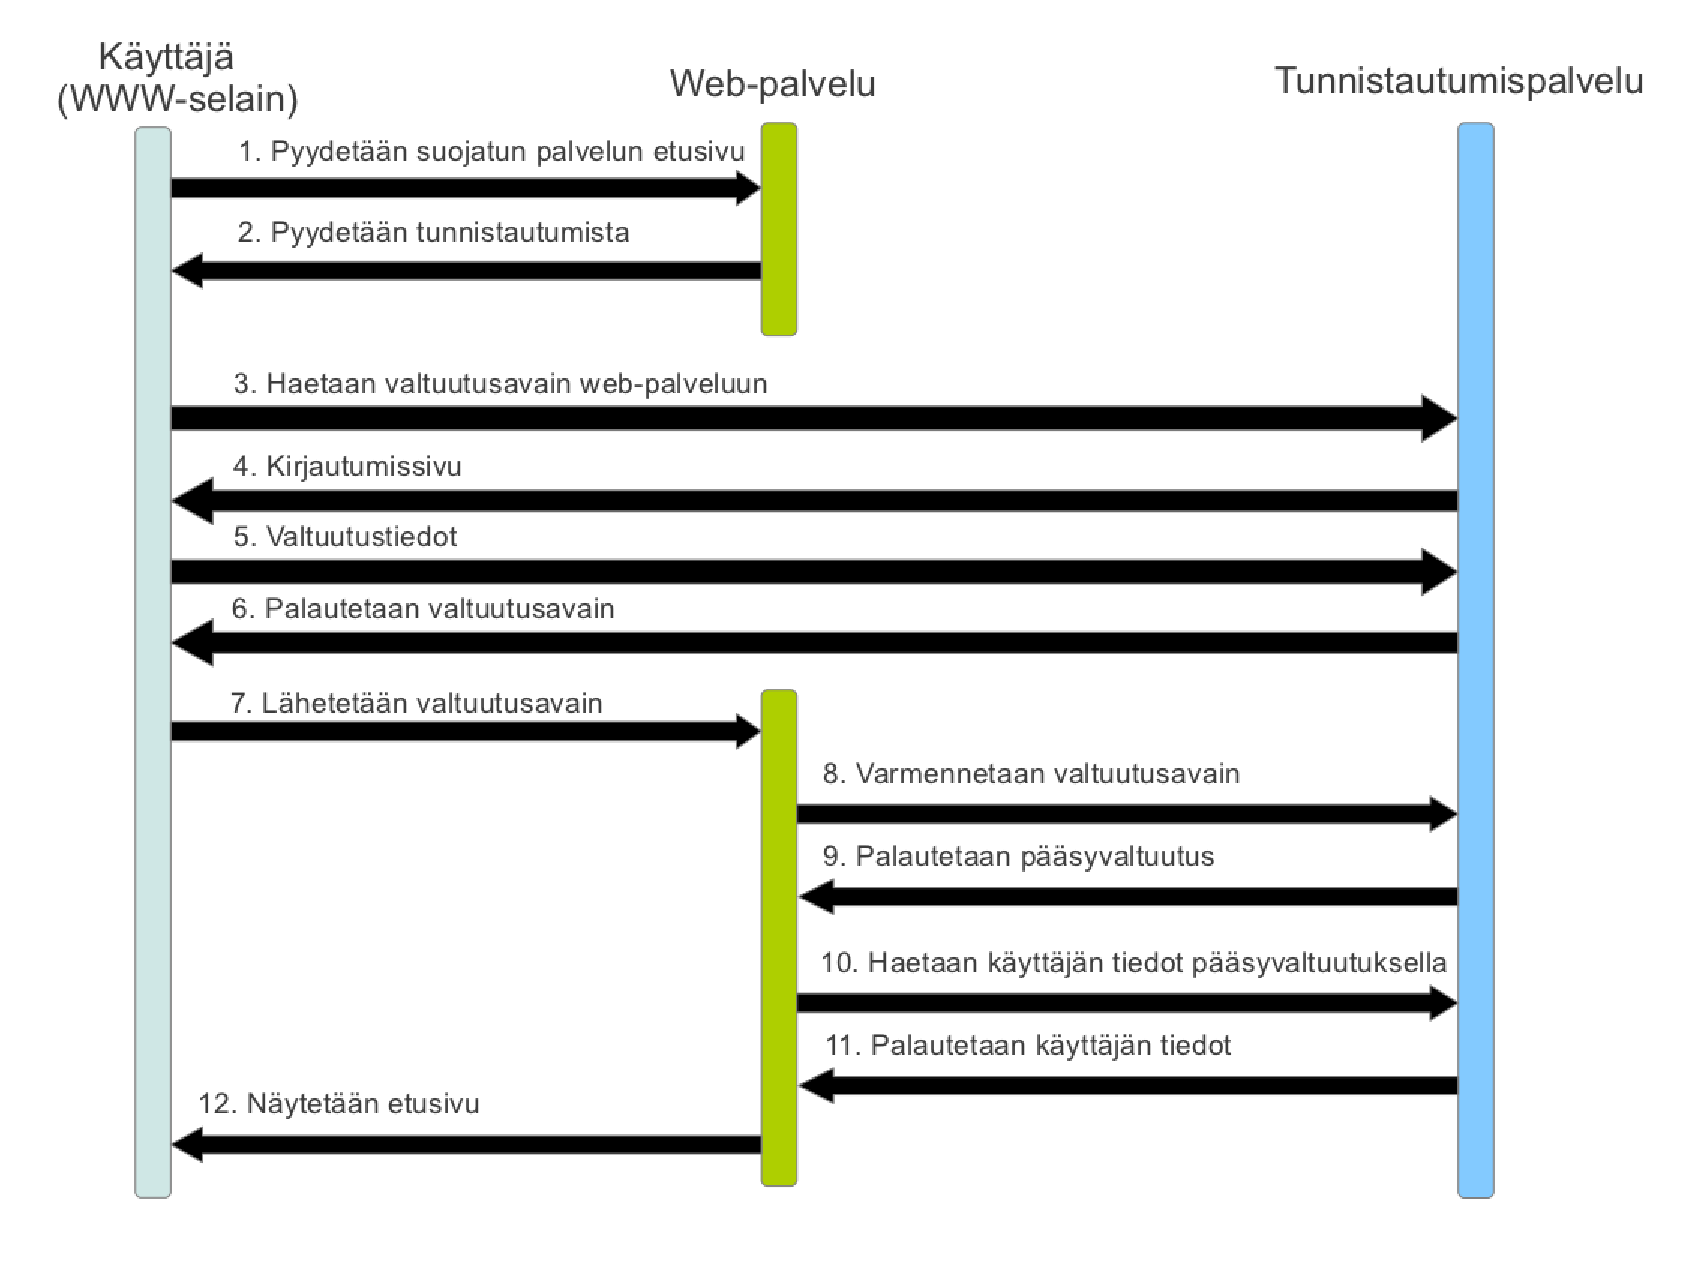
\includegraphics[width=\textwidth]{teknologiat/protokollat/oauth.eps}
\caption{OAuthin toiminta sekvenssikaaviona.}%
\label{oauth}
\end{figure}

OAuthissa valtuutusavaimelle voidaan asettaa erilaisia rajoituksia esimerkiksi sen suhteen, mitä tietoja käyttäjästä annetaan web-sovellukselle tai mihin resursseihin kyseisellä avaimella pääsee käsiksi. Kuvassa \ref{facebook_login} kirjautumisen yhteydessä Porkkanamafialle annetaan oikeus nähdä käyttäjän nimi, profiilikuva, sukupuoli jne. OAuth ei siis ole varsinaisesti tunnistautumisprotokolla, mutta valtuutusavaimen perusteella käyttäjä voidaan yksilöidä: kun käyttäjä kirjautuu myöhemmin uudestaan Porkkanamafiaan, hän hakee valtuutusavaimen Facebookilta, jota käyttämällä Porkkanamafia hakee Facebookista käyttäjän tiedot. Käyttäjän tiedoissa mukana olevalla Facebookin yksilöivällä tunnistenumerolla käyttäjä voidaan todeta samaksi kuin edellisellä kirjautumiskerralla.
\subsection{Yhteenveto}
Keskitetyn tunnistautumispalvelun käyttö on perusteltua, jos ympäristössä on useita käyttäjän tunnistamista vaativia web-sovelluksia. Tunnistautumispalvelun käytöllä ehkäistään käyttäjätietojen kopiointiin liittyviä synkronointiongelmia, kun käyttäjädata on keskitetty yhteen paikkaan. Erityisesti arkaluontoinen data, kuten salasanatiivisteet, kannattaa keskittää, jolloin ne eivät päädy vääriin käsiin yksittäisiin web-sovelluksiin kohdistuneiden tietomurtojen yhteydessä.

Tunnistautumispalvelu mahdollistaa myös muiden kuin järjestelmän ylläpitäjien tuottamien sovellusten käytön organisaation sisäisillä käyttäjätunnuksilla. Käyttämällä luotettavaksi todettuja rajapintoja, voi ylläpito antaa kolmannen osapuolen toteuttamalle web-sovellukselle oikeuden käyttää tunnistautumispalvelua käyttäjän tunnistamiseen. Tällöin käyttäjä ohjataan tunnistautumispalveluun tunnistamisen ajaksi ja web-sovellus saa vain pääsyvaltuuden, jolla sovellus voi hakea käyttäjän tiedot. Käyttäjän tunnistetiedot eivät tule missään vaiheessa tunnistamista tarvitsevan web-sovelluksen tietoon. Näin ollen esimerkiksi Facebook-tunnuksilla voi kirjautua useaan web-sovellukseen, vaikka Facebookilla ei ole tarkkaa tietoa sovelluksien sisäisestä toimintalogiikasta.

Tutkielmassa esitellyn Kapsi ry:n hallintatyökalujen tapauksessa palvelu tullaan toteuttamaan Django-sovelluskehyksellä, mutta myös valmiita toteutuksia on olemassa eri intranet-ympäristöihin. Teknologivalinta tulee tehdä sovellusympäristön mukaan, eikä yksi ratkaisu sovi kaikkiin ympäristöihin. Web-sovelluksen ja tunnistautumispalvelun välinen rajapinta pitää huolen palveluiden yhteensopivuudesta. Rajapinnoiksi on valittavissa useita eri protokollia, kuten Web Services -standardin SAML tai avoimen lähdekoodin yhteisössä syntyneet OpenID ja OAuth. Protokollien käyttö rinnakkain on myös mahdollista, jolloin tunnistautuminen voidaan tehdä esimerkiksi SAML- tai OAuth-protokollalla riippuen web-sovelluksesta.

Tunnistautumiseen liittyvien tehtävien erottaminen yksittäisiltä web-sovelluksilta erillisen palvelun tehtäväksi on palvelusuuntauneiden arkkitehtuurien periaatteiden mukaista. Tällaisten arkkitehtuurien mukaan toteutetuissa sovellusympäristöissä jokaisella web-sovelluksella on oma tarkasti määritelty tehtävä. Kun arkkitehtuurissa on oma palvelu tunnistautumiselle, on pienten yksittäisten komponenttien toteutus helpompaa, koska jokaisen komponentin kohdalla ei tarvitse huolehtia tunnistautumisen toteutuksesta.

Web-sovelluksen ja tunnistamisen erottaminen toisistaan mahdollistaa myös tunnistautumisen tehostamisen ilman muutoksia web-sovellusten toimintaan. Järjestelmässä voidaan ottaa salasanan lisäksi käyttöön toiseen tekijään perustuva tunnistaminen, jolloin esimerkiksi käyttäjän täytyy salasanan lisäksi syöttää matkapuhelimeen lähetetty tunnistekoodi. Web-sovelluksen ja tunnistautumispalvelun välinen rajapinta ei tässä tapauksessa muutu, joten tunnistamisen parantaminen ei edellytä web-sovelluksien muuttamista.

Keskitetyn pääsynvalvonnan toteuttaminen tutkielmassa kuvatuilla periaatteilla on mahdollista. Tällöin tiedot käyttäjien pääsyoikeuksista ympäristön sisällä ovat yhdessä paikassa, joka helpottaa niiden hallinnointia. Esimerkiksi henkilön siirtyessä tehtävästä toiseen, voidaan hänen pääsyvaltuudet muuttaa samasta paikasta. Pääsynvalvontaan voidaan käyttää esimerkiksi tutkielmassa esiteltyjä SAML- tai OAuth-protokollia.

Käyttäjän tunnistamista vaativissa web-sovelluksissa käyttäjän tunnistaminen kannattaa toteuttaa erillisenä komponenttina. Käytettyjen teknologioiden suhteen valinta täytyy tehdä web-sovellusympäristön mukaan, koska kaikkiin ympäristöihin sopivaa ratkaisua ei ole. Tässä tutkielmassa esitellyt periaatteet ovat kuitenkin sovellettavissa eri teknologioita käytettäessä.
